\documentclass{article}
\usepackage{cmap}
\usepackage{multicol}
\usepackage[top=3cm,bottom=3cm,left=3cm,right=3cm]{geometry}
\usepackage{hyperref}
\usepackage{graphicx}
\usepackage{caption}
\usepackage{capt-of}
\newenvironment{Figure}
  {\par\medskip\noindent\minipage{\linewidth}}
  {\endminipage\par\medskip}

\title{Forrest Fire Simulation model}
\author{Tom Peerdeman - 10266185 \& Ren\'e Aparicio Saez - 10214054}

\begin{document}

\maketitle

\begin{abstract}
\textbf{Le Abstract.}
\end{abstract}

\begin{multicols}{2}

\subsection*{Introduction}
Forest fires can spread in various ways and can be effected by a lot of environmental variables. Some variables are straight forward, as seen in the forest fire simulation made by Peerdeman, cite hier. Different neighborhoods and the density of a forrest are not just the only variables defining the spread of a forest fire. The way a fire spreads between flammable objects for example can make a huge difference in the way a forest fire moves. Fire can also be affected by environmental variables, like water, the weather or wind. Manmade objects and people can interfere with the fire as well. Fire fighters can try to extinguish fire to keep the fire from spreading. Paths and roads, like water cannot be set on fire. It is however possible for fire to cross roads and some streams of water if the conditions are right. All these variables have to be taken into account when simulating a forest fire.\\\\
The experiments done in this paper are an expansion of the work done by Peerdeman,le cite hier. The forest fire simulations are done by using cellular automata. Instead of using rules as was the case in the previous experiments, the experiments posed for this paper require probabilities. These probabilities are needed to simulate the environmental effects on the forest fire. 

\subsection*{Defining the neighborhoods}
\subsubsection*{Different grids}
In order to ensure that the simulation is applicable in many situations, three different types of grids were used to simulate forest fires. These grids are: the Cartesian grid, the hexagonal grid and the triangular grid. Each grid has a different spread of fire.\\\\
For the Cartesian grid a straightforward method is used. By using a Moore neighborhood the eight squares around the current square can be directly influenced. The neighborhood is shown in figure \ref{fig:cartesianstd}.\\\\
The hexagonal grid could be positioned in two different ways. Either with points facing up and down, or with points facing left and right. Both types of hexagons will do, by changing your perspective on the simulation, it is possible to simulate the other type of hexagon. For the experiments and simulations the type with points to the top and bottom is used. As shown by Hernandez et al. \cite{HernandezEncinas20071213}, hexagonal grids show a slight difference in mathematics when they are either odd or even (in this case along the x-axis). The neighborhood is shown in figure \ref{fig:hexstd}.  \\\\
Just like the hexagonal grid, the triangular grid can be placed in two different ways. Either with two of the points along the x-axis or two points along the y-axis. The first type is chosen, to keep consistency for all grids. Whereas the fire spread of the Cartesian and the hexagonal grids are the same, no matter the location, the spread of the triangular grid differs per position. The triangle can either point up or down, switching along each axis. The neighborhoods for the triangles are shown in figure \ref{fig:triangle1std} and figure \ref{fig:triangle2std}.
\begin{Figure}
 \centering
 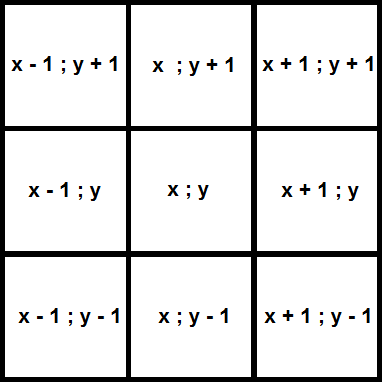
\includegraphics[width=0.79\textwidth]{imgs/cartesian.png}
 \captionof{figure}{Cartesian grid neighborhood}
\label{fig:cartesianstd}
\end{Figure}
\begin{Figure}
 \centering
 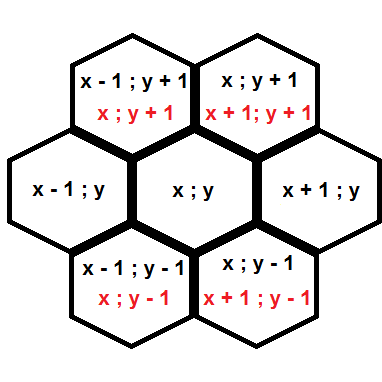
\includegraphics[width=0.79\textwidth]{imgs/hexagonal.png}
 \captionof{figure}{Hexagonal grid neighborhood}
\label{fig:hexstd}
\end{Figure}
\begin{Figure}
 \centering
 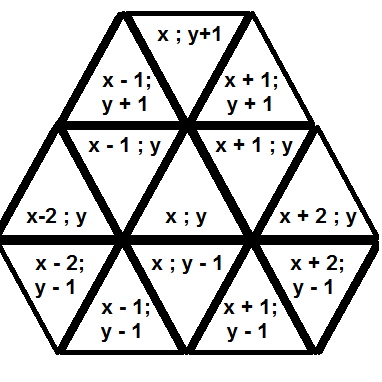
\includegraphics[width=0.79\textwidth]{imgs/triangle1.png}
 \captionof{figure}{Triangle 1 grid neighborhood}
\label{fig:triangle1std}
\end{Figure}
\begin{Figure}
 \centering
 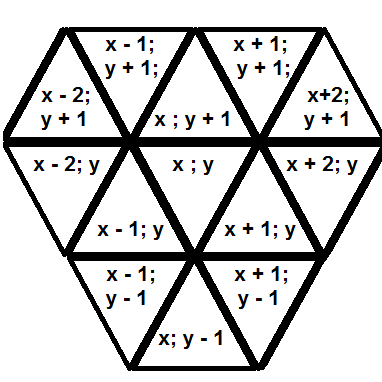
\includegraphics[width=0.79\textwidth]{imgs/triangle2.png}
 \captionof{figure}{Triangle 2 grid neighborhood}
\label{fig:triangle2std}
\end{Figure}

\subsubsection*{Spread probabilities}
Each grid can be initialized with certain probabilities for their neighborhoods. These probabilities represent the probability of fire to spread to the specific cell. By using probabilities, instead of a guaranteed fire spread, different types of situations can be used when simulating the fire. By changing the probabilities in certain ways, different types of weather, wind and terrain can be simulated. For example, when the weather is rainy, the probabilities can be set lower, while when it’s hot the probabilities can be set higher. The same goes for wind, if the wind blows in a certain direction, the probabilities for that direction can be set higher than the other directions.\\\\
In order to increase the environmental factor even more, it is also possible to influence cell's outside the neighborhood. In this way, extreme hot weather or high wind speeds can be simulated even better. When this feature is used, a new probability is created for fire to spread to a cell with a distance of two cell's from the current cell. This probability is calculated by dividing the interpolated probabilities of the cell's in the neighborhood in the direction of the cell outside the neighborhood by a given number. This way, the probability for fire to spread is always equal or lower to the probabilities of the cell's its probability was interpolated from.\\
The areas that could catch fire if the spread of distance two is enabled is shown in the following figures. Note that the area of the triangles is a bit odd. The area that would have been able to get on fire if all the surrounding cell's were used, was too big in comparison to the other grids. Because of that the area for the triangles has been reduced. The extended neighborhoods are shown in gray in figures \ref{fig:extcartesianstd},  \ref{fig:exthexstd},  \ref{fig:exttriangle1std} and  \ref{fig:exttriangle2std}.\\\\
Besides the increased environmental factor, the extended neighborhood also has as advantage that it can simulate fire moving across water and paths. This is a very useful feature. If this wasn't the case, fire could never spread even when facing a small river or path.
\begin{Figure}
 \centering
 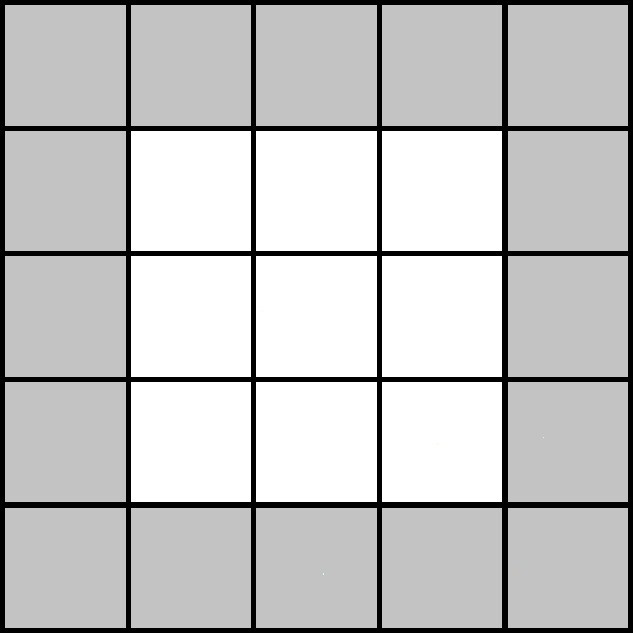
\includegraphics[width=0.79\textwidth]{imgs/extendedcartesian.png}
 \captionof{figure}{Extended Cartesian grid neighborhood}
\label{fig:extcartesianstd}
\end{Figure}
\begin{Figure}
 \centering
 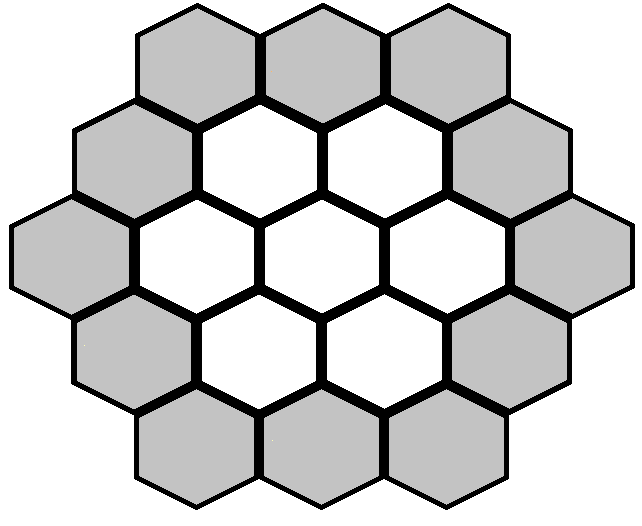
\includegraphics[width=0.79\textwidth]{imgs/extendedhexagonal.png}
 \captionof{figure}{Extended Hexagonal grid neighborhood}
\label{fig:exthexstd}
\end{Figure}
\begin{Figure}
 \centering
 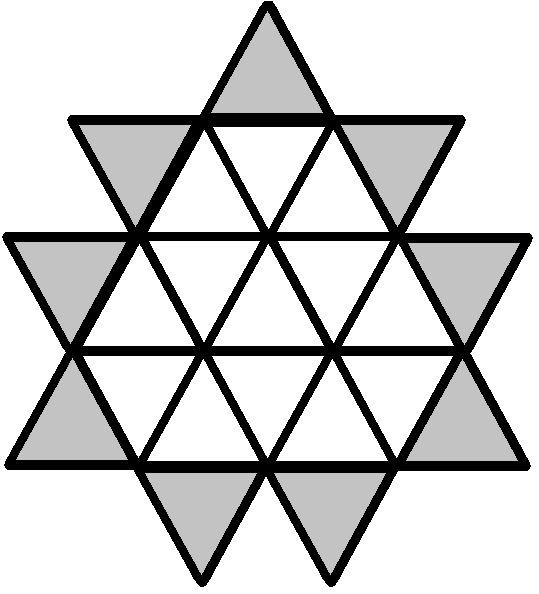
\includegraphics[width=0.79\textwidth]{imgs/extendedtriangle1.png}
 \captionof{figure}{Extended Triangle 1 grid neighborhood}
\label{fig:exttriangle1std}
\end{Figure}
\begin{Figure}
 \centering
 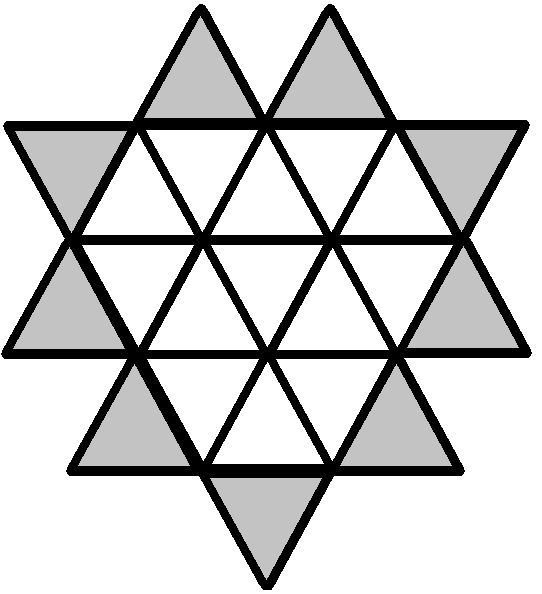
\includegraphics[width=0.79\textwidth]{imgs/extendedtriangle2.png}
 \captionof{figure}{Extended Triangle 2 grid neighborhood}
\label{fig:exttriangle2std}
\end{Figure}

\subsection*{Experiments}
In addition to the experiments already made for the Cartesian grid, the same experiments have to be done for the other grids. Besides reproducing the same experiments for the other grids, new experiments can be done. The new variables create a huge variety in possible experiments. To expand the made experiments, the most logical addition is to gradually add variables and to look at the impact of these variables on the known results.\\\\

\subsubsection*{Basic experiments}
To start off, results are needed for a simulation on a simple forest, without any roads or streams of water running through the forest. Even though the results for the Cartesian grid are already known the experiments are made for all the grids, to ensure consistency in the experiments. Each simulation is run 50 times. This is done to overcome coincidental spreads and to show a more generalized view for each result.\\\\
By increasing the density gradually after each run of simulations a variety of information van be analyzed. It is possible to look at the percentage of the forest that is burned, how long the fire burned and how long it took for the fire to reach the other side of the grid.

\subsubsection*{Additional Experiments}
After the basic experiments are done, variables can be added to the simulations. The first variable to be added is the enlarged distance for fire to spread to more neighbors. This variable will increase the speed of the fire. Again the density is increased after every set of simulation runs.\\\\
The second variables to be added are roads and streams of water. These variables are tested with and without the additional distance for fire to spread. Without the additional distance, the addition of roads and water will most likely bring on problems for the simulation. Fire cannot spread across water or roads if it isn't allowed to move an extra square to each side. This will change when the additional distance is enabled again.\\\\
After these experiments are done, there is a final variable, the fire fighters, that could change the spread of fire. Again two experiments have to be made, one with and one without the additional distance. With these final experiments a conclusion can be made about the impact of each variable on the spread of fire.

\subsubsection*{Expected results}
It is expected that the fire will spread the fastest for the grid with the most neighbors. The amount of neighbors depends on the additional distance that is used for some experiments. As shown, the Cartesian grid has 9 neighbors directly surrounding the cell. If the distance is increased, the number of neighbors increases to 27 neighbors that can catch fire. For the hexagonal grid this is 6 neighbors directly surrounding the cell and a total of 18 when the distance is increased. Finally the neighborhood of the triangular grid starts with 12 neighbors directly surrounding the cell and 21 neighbors with an increased distance.\\\\
As can be seen from the amount of neighbors it is expected that, without the additional distance, the triangular grid will have the fastest spread of fire, followed by the Cartesian grid and the hexagonal grid. When the distance is increased, the amount of neighbors for the Cartesian grid increases more than the amount of neighbors for the other grids. Because of this is can be expected that the Cartesian grid will move faster with the increased distance enabled, followed by the triangular grid and the hexagonal grid being the slowest.\\\\
It is also expected that the percentage of forest that will burn down will depend on the amount of neighbors surrounding a cell. Therefore a coherence is expected in the percentage of the forest that is burned and the speed the forest fire will spread.\\\\
Besides the additional distance variable, the addition of roads and streams of water will affect the speed of the fire spread as well. By adding roads and streams of water, the fire will be slowed down. Depending on the distance the fire can travel from a cell, the fire will either be stopped by the roads and water or slowed down by the fact that the probability to cross the water or the road is lower then moving to a cell closer to the current cell. It can therefore be expected that the addition of water will drastically interfere with the speed and the percentage of the forest that is burnt when the fire can only spread to the direct neighbors. If the distance the fire can spread to is increased it can be expected that the fire will move a bit slower, but the percentage that will get burned down will remain around the same as without water or roads.\\\\
The final variable, the firefighters, will interfere with the spread of fire and the percentage that will get burned. When just the surrounding cells can be set on fire, the firefighters will most likely lower the percentage of the forest that will get burned down. The fire will spread less fast when facing fire fighters as well. However, because firefighters will only spawn when roads are around, the fire will get stopped by the roads anyway. Therefore the firefighters will not provide a very big impact, compared to the same experiment without the firefighters.\\\\
When the firefighters are added and the additional distance is used, the fire will again be slowed down and a lower percentage of the forest will get burned down. However, the fire will most likely still burn down a large amount of forest, due to the bigger area a fire can spread to compared to the slow speed a fire fighter can move towards a fire. It is therefore expected that a firefighter only has a small impact on the speed of the fire and percentage of forest that will get burned down.


\subsection*{Results}
\subsection*{Interpretation}

\subsection*{Discussion \& Conclusion}

\nocite{*}
\bibliographystyle{plain}
\bibliography{Forest_fire_paper}
\end{multicols}

\end{document}
